\Chapter{Koncepció}

\Section{A fejezet célja}

A szimulációs környezet inspirációt vesz már elkészített videójátékokból, mint például a \textit{Pixel Dungeon} \cite{pixeldungeon} és \textit{Darkest Dungeon} \cite{darkestdungeon} 
nevű játékokból ismerhető szoba és folyosó kapcsolat. Ahol minden szobát egy folyosó köt össze egy másik tetszőleges szobával.
A Darkest Dungeon-hoz képest a játékmenet rugalmasabb, mivel a szobák bármikor elhagyhatóak és megközelíthetőek, ha engedi azt a pálya jelenlegi belső felépítése.
Azaz, ha nincs útban valami, ami megakadályozza.

A fent említett két játék mind körökre osztott, ahogyan a szimulációs környezetünk is az lesz.

A szimulációs környezetünk viszont egyedi lesz abból a szempontból, hogy az ágensek csoportokra vannak osztva és közös céllal
rendelkezve próbálják legyőzni egymást és az ellenséges ágenseket.

Az alkalmazás a \textit{Pela} fantázia nevet kapta.

\Section{Felhasznált technológiák}

\subsection{Java}

A Java általános célú, objektumorientált programozási nyelv, amelyet a Sun Microsystems fejlesztett a 90-es évek elejétől kezdve egészen 2009-ig, amikor a céget felvásárolta az Oracle \cite{arnold2005java}.

\subsection{Java Swing}

A Swing osztályok kiküszöbölik a Java legnagyobb gyengeségét, a viszonylag primitív felhasználói felület eszközkészletét. A Java Swing segít a Swing osztályok teljes előnyeinek kihasználásában,
részletes leírást adva minden osztályról és felületről a kulcsfontosságú Swing csomagokban \cite{10.5555/291162}.

\Section{Az ágens szimulációs felület elemei}

Az ágensek és környezetük szimulációjához, a rajtuk elvégzendő mérésekhez célszerű összerakni egy grafikus felületet. A következő szakaszokban ezeknek a két fő elemét, a menüt és az UI-t mutatja be a dolgozat.

\SubSection{Menü}

A szimulációs környezethez tartozik egy menü ablak. Ennek elemei az alábbiak.

\medskip

\noindent Szimuláció indítása előtt:
\begin{itemize}
    \item Középen felül a \textit{Main Menu} kiírását láhatjuk, alatta pedig 2 opcióból választhatunk (\ref{fig:MainMenu}. ábra):
    \begin{itemize}
    \item[(1)] \textit{Start}, a kiválasztása esetén elindul a szimuláció,
    \item[(2)] \textit{Quit}, a szimulációs ablak bezárása.
    \end{itemize}
    \item A fenn említett két menüpont között a \texttt{W} (fel) és \texttt{S} (le) billentyűk lenyomásával navigálhatunk.
    \item Aláhúzva jelzi a felhasználónak, hogy mely menüpont van éppen kiválasztva.
    \item A különböző ablakok és UI elemek egy egyedi fontot használnak \cite{yosterislandfont}.
\end{itemize}

\noindent A szimuláció megállítása esetén:

\begin{itemize}
    \item A szimulációban a \texttt{P} billentyű lenyomásával képes a felhasználó megállítani a szimuláció menetét.
    \item A megállítást a bal felső sarokban kiírt fehér \textit{Paused} kiírás jelzi a felhasználó számára (\ref{fig:Paused}. ábra).
    \item Ilyenkor az ágensek nem kapnak lehetőséget a lépésre, de a felhasználó képes a kamera mozgatására a nyilak segítségével.
    \item A felhasználó szintén képes az ágensek \textit{Statistics} ablakát megnyitni/bezárni a \texttt{C} billentyű megnyomásával, és előre/hátra lapozni az ágensek között a \texttt{Q} (balra) és \texttt{E} (jobbra) billentyűk megnyomásával, ha több van a szimulációban, mint 1.
    \item Ugyanígy képes megnyitni/bezárni az adott ágenshez tartozó \textit{Inventory} ablakot az \texttt{I} billentyű megnyomásával, ha látszódik az ágens statisztikája ablak.
    \item A \texttt{P} billentyű újonnan megnyomásával ott folytatódik a szimuláció, ahol abbamaradt (\ref{fig:nonPaused}. ábra).
\end{itemize}

\Section{UI}
\label{UI}

A UI (\textit{User Interface}) foglalja magába az ágens szimulátor fő elemeit. A következőkben ennek az elemei, azok funkciói kerülnek felsorolásra.

\medskip

\noindent A szimuláció figyelésére szolgáló UI ablakok, amelyek a szimuláció kezdete után a képernyőn jelennek meg, a következők:

\begin{itemize}
    \item \textit{Statistics}: A \texttt{C} billentyű megnyomására megjelenik az első számú ágens Statistics ablaka (\ref{fig:Statistics}. ábra).
    \item \textit{Inventory}: Az \texttt{I} billentyű megnyomására megjelenik az az adott ágens Inventory oldala (\ref{fig:Inventory}. ábra).
\end{itemize}

\noindent Statistics

\begin{itemize}
    \item Egy adott ágens adatának a kiolvasásának az eredményeit megjelenítő UI ablak. 
    \item A szimulációban megállítástól függetlenül a \texttt{C} billentyű megnyomására jelenik meg és tűnik el.
    \item Megnyitásakor mindig a még szimulációban létező ágensek közül az első számú ágens adait fogja visszaadni.
    \item A vizsgálandó ágens elpusztulásakor a még létező ágensek közül az új első számú ágens adatait fogja visszaadni.
    \item Ezen az ablakon a következő ágens adatokat írja ki:
    \begin{itemize}
    \item \textit{Sorszám}: Az ágens sorszámát adja vissza.
    \item \textit{HP} (életerő): Az ágens aktuális életerejét adja vissza.
    \item \textit{Erő} (str) Az ágens aktuális str értékét adja vissza.
    \item \textit{Kitartás} (vit): Az ágens aktuális vit értékét adja vissza.
    \item \textit{Kitérés} (eva): Az ágens aktuális eva értékét adja vissza.
    \item \textit{Pontosság} (acc): Az ágens aktuális acc értékét adja vissza.
    \end{itemize}
    Ezek a számok változhatnak az alapján, hogy milyen felszerelést hord az adott ágens.
    \item Új tárgy felvételénél, ha úgy ítéli, hogy jobb, mint az általa hordott azonos típusú tárgy, akkor lecseréli, és ennek megfelelően frissülnek a statisztikái.
\end{itemize}

\noindent Inventory

\begin{itemize}
    \item Nem nyitható meg, ha nincs még megnyitva egy tetszőleges ágens \textit{Statistics} ablaka (\ref{fig:Inventory}. ábra).
    \item Megnyitásakor annak az ágensnek az \textit{Inventory}-ja lesz látható, amelyiknek a \textit{Statistics} oldala nyitva van.
    \item A \textit{Statistics} oldalon az előre/hátra lépés esetén az \textit{Inventory} az újonnan szemügyre vett ágens \textit{Inventory}-ját fogja megjeleníteni a felhasználó számára.
    \item Az \textit{Inventory}-ban a következő típusú tárgyak találhatóak meg:
    \begin{itemize}
    \item \textit{Armor} (páncél): Páncélként hordható tárgy, 4 alapstatisztikát tartalmaz.
    \item \textit{Helmet} (sisak): Sisakként hordható tárgy, 4 alapstatisztikát tartalmaz.
    \item \textit{Weapon} (fegyver): Fegyverként hordható tárgy, 4 alapstatisztikát tartalmaz.
    \item \textit{Key} (kulcs): Ajtó kinyitásához szükséges tárgy.
    \end{itemize}
    \item Az \textit{Inventory}-ban a \texttt{WASD} billentyűk lenyomásával választhatjuk ki, hogy mely \textit{Inventory} helyet akarjuk megnézni.
    \item A fehér üres négyzet jelöli azt a helyett az \textit{Inventory}-ban, amelyet éppen szemügyre vesz a felhasználó.
    \item Ha felszerelés típusú az adott tárgy, akkor a nevét és a 4 alapstatisztika értékét írja ki.
    \item Ha nem felszerelés típusú az adott tárgy, akkor pedig a nevét írja ki.
\end{itemize}

\noindent Életcsík

\begin{itemize}
    \item Minden ágens fölött az aktuális életcsíkja jelenik meg automatikusan.
\end{itemize}


\Section{Szimulációs környezet specifikálása}

A következőkben a szimulációs környezet modelljének, elemeinek a specifikálására kerül sor.

\subsection{Map}

A szimulációban az ágensek egy diszkrét négyzetrács felbontáson tudnak mozogni. Ennek a mérete rögzített, $50 \times 50$, és minden elemhez egy saját definiálású \texttt{block} típus tartozik.

Egy \texttt{block}-nak van típusa, amely egy egész számként reprezentálható. Ez a következő értékeket veheti fel:
\begin{itemize}
\item 0 típus: Üres, a \textit{map}-on nem elérhető területeket jelöli.
\item 1 típus: Fal, a bejárható területeket körbezáró fal, amelyen nem lehet átmenni.
\item 2 típus: Füves terület, az ágensek által bejárható területek.
\end{itemize}

Az $50 \times 50$-es mátrixon minden 2-es típusú blokkra helyezhetünk el egy objektumot. Az objektumok típusai az alábbiak lehetnek.

\begin{itemize}
\item \textit{Brick}: Egy mozgást korlátozó objektum. Nincs különösebb szerepe.
\item \textit{Chest}: \textit{End screen}-t előidéző tárgy, amely a szimuláció végét jelenti.
\item \textit{Door}: Egy mozgást korlátozó objektum. Kulccsal kinyitható az ágensek által.
\end{itemize}

Az objektumok egy részhalmaza olyan, hogy az ágensek fel tudják azokat venni az Inventory-jukba, amelyek nem korlátozzák a mozgást. Ezek az alábbiak:
\begin{itemize}
\item \textit{Key},
\item \textit{Entity\_Armor\_01},
\item \textit{Entity\_Weapon\_01},
\item \textit{Entity\_Helmet\_01},
\item \textit{Entity\_Armor\_02},
\item \textit{Entity\_Weapon\_02},
\item \textit{Entity\_Helmet\_02}.
\end{itemize}

Szimuláció kezdetekor megtörténik a \textit{map} beolvasása. Ezt követően minden 2-es típusú blockra helyezhetünk el egy ágenst.
\begin{itemize}
    \item \textit{EntityFaction0}: 0-es számú csapatban lévő ágens.
    \item \textit{EntityFaction1}: 1-es számú csapatban lévő ágens.
\end{itemize}

A szimulációs környezetben adott számú elemet helyezünk le. Konkrétan az alábbi számú és típusú elemek kerülnek rá:
\begin{itemize}
    \item 18 szoba, 
    \item 25 ajtó,
    \item 25 kulcs,
    \item 4 ágens,
    \item 10 felvehető tárgy,
    \item 2 chest,
    \item 12 brick.
\end{itemize}

\SubSection{Szobák és folyosók}

A \textit{map}-en szobák és folyosók alakíthatók ki, de nem tetszőleges módon. Az alábbi szabályrendszer írja le, hogy milyen feltételek szerint helyezheti le ezeket a program.
\begin{itemize}
\item A szobákat több szomszédos cellák alkotják.
\item A szobákat folyosók kötik össze, amelyeket pontosan kettő cellával szomszédos cellák alkotnak.
\item Minden szomszédos szobát egy ajtó választ el egymástól.
\item A szobák celláin korlátozottan helyezkedhetnek el oszlopok, amely a cellát nem bejárható cellává alakítja át, és korlátozza a látást.
\item Minden szoba tartalmaz legalább 1 kulcsot, amely elősegíti a \textit{map} bejárhatóságát az ágensek által.
\end{itemize}

\SubSection{További map-re vonatkozó szabályok}

A \textit{map} szobák és folyosók összessége, ahol a szobák alakjánál törekszünk a négyzet alakú szobák elkerülésére. A folyosók általában rövidek és egy szobából akár több is nyílhat egy adott szobára.
A \textit{map} blokkokból épül fel. Blokkok típusát egy $[0, 2]$ intervallumon belüli számok jelölik.
Ezek az adatok a szimuláció kezdetekor kerülnek beolvasásra a \texttt{world01.txt}-ből.

A szobákban és a folyosókban bejárható terület egy mátrixhoz hasonló, amely celláit blokkoknak nevezzük.

Minden blokkhoz tartoznak további adatok, úgy mint:
\begin{itemize}
    \item $X$ koordináta (Integer),
    \item $Y$ koordináta (Integer).
\end{itemize}

\noindent Fontosabb kizáró feltételek:
\begin{itemize}
    \item Ajtó csak szoba és a folyosó, vagy szoba és a szoba között létezzen.
    \item Folyosóból ne nyíljon ajtó folyosóra.
    \item Két különböző folyosó ne érjen össze.
    \item Nem lehet olyan cellára mozgást kizáró objektumokat letenni, amely lehetetlenné teszi a \textit{map} egy tetszőleges pontjáról a \textit{map} egy másik tetszőleges pontjára való eljutását.
\end{itemize}

\Section{Tárgyak}

A tárgyakhoz a következő fontosabb adatok tartoznak:
\begin{itemize}
    \item \textit{name} (String),
    \item \textit{typeName} (String),
    \item \textit{type} (Integer),
    \item \textit{str} (Integer),
    \item \textit{vit} (Integer),
    \item \textit{eva} (Integer),
    \item \textit{acc} (Integer).
\end{itemize}

\SubSection{name}

Az adott tárgyat bemutató név.

\subsection{typeName}

A tárgyak tartalmaznak tárgy típus nevet, például: Armor, Helmet, Key... stb.

\subsection{type}

A Key tárgy a "0" típusú, amíg minden hordható tárgy a "2" típus számot tartalmazza.

\subsection{str}

Ha az adott tárgy az ágensek által hordható tárgy, azaz nem kulcs, van valós str értéke.

\subsection{vit}

Ha az adott tárgy az ágensek által hordható tárgy, azaz nem kulcs, van valós vit értéke.

\subsection{eva}

Ha az adott tárgy az ágensek által hordható tárgy, azaz nem kulcs, van valós eva értéke.

\subsection{acc}

Ha az adott tárgy az ágensek által hordható tárgy, azaz nem kulcs, van valós acc értéke.

\Section{Tárgy nevek}

\SubSection{Entity\_Helmet\_01}

Ágens által használható felszerelési tárgy, amely statisztikát ad, amelyek hozzáadódnak, illetve kivonódnak az ágens jelenlegi statisztikáiból.

\begin{itemize}
    \item Erő (str): [1,3[
    \item Kitartás (vit): [1,3[
    \item Kitérés (eva): [1,3[
    \item Pontosság (acc): [1,3[
\end{itemize}

\SubSection{Entity\_Helmet\_02}


Ágens által használható felszerelési tárgy, amely statisztikát ad, amelyek hozzáadódnak, illetve kivonódnak az ágens jelenlegi statisztikáiból.

\begin{itemize}
    \item Erő (str): [0,4[
    \item Kitartás (vit): [0,4[
    \item Kitérés (eva): [0,4[
    \item Pontosság (acc): [0,4[
\end{itemize}

\SubSection{Entity\_Armor\_01}

Ágens által használható felszerelési tárgy, amely statisztikát ad, amelyek hozzáadódnak, illetve kivonódnak az ágens jelenlegi statisztikáiból.

\begin{itemize}
    \item Erő (str): [1,3[
    \item Kitartás (vit): [1,3[
    \item Kitérés (eva): [1,3[
    \item Pontosság (acc): [1,3[
\end{itemize}

\SubSection{Entity Armor 02}


Ágens által használható felszerelési tárgy, amely statisztikát ad, amelyek hozzáadódnak, illetve kivonódnak az ágens jelenlegi statisztikáiból.

\begin{itemize}
    \item Erő (str): [0,4[
    \item Kitartás (vit): [0,4[
    \item Kitérés (eva): [0,4[
    \item Pontosság (acc): [0,4[
\end{itemize}

\SubSection{Entity Weapon 01}

Ágens által használható felszerelési tárgy, amely statisztikát ad, amelyek hozzáadódnak, illetve kivonódnak az ágens jelenlegi statisztikáiból.

\begin{itemize}
    \item Erő (str): [1,3[
    \item Kitartás (vit): [1,3[
    \item Kitérés (eva): [1,3[
    \item Pontosság (acc): [1,3[
\end{itemize}

\SubSection{Entity Weapon 02}

Ágens által használható felszerelési tárgy, amely statisztikát ad, amelyek hozzáadódnak, illetve kivonódnak az ágens jelenlegi statisztikáiból.

\begin{itemize}
    \item Erő (str): [0,4[
    \item Kitartás (vit): [0,4[
    \item Kitérés (eva): [0,4[
    \item Pontosság (acc): [0,4[
\end{itemize}

\SubSection{Kulcs}

Celláról szerezhetőek meg.
Szerepük az ajtók kinyitása az ágens által.
Kulcsot tartalmazó ágens, elpusztulásakor a legutolsó helyén hagyja a kulcsot.

\Section{Ágensek}

\subsection{Statisztika}
\label{statisztika}
\begin{itemize}
    \item Ágensek 4 alap statisztikával rendelkeznek.
    \item Ez a 4 statisztika a következők: Erő, Kitérés, Kitartás, Pontosság.
    \item Az ágensek kezdő statisztikája fix 1.
\end{itemize}

\noindent A következő tárgyakkal kezd a szimulációban:

\begin{itemize}
    \item Entity Helm 01,
    \item Entity Armor 01,
    \item Entity Weapon 01.
\end{itemize}

\subsection{Sebzés számlálás}

\label{számlálás}

A támadásnak két végkimenetele lehet:

\begin{itemize}
    \item Találat,
    \item Eltévesztve.
\end{itemize}

\noindent Találat esetén, kiszámolódik a sebzés mértéke. 

\noindent Eltévesztés esetén nem történik meg a sebzés. 

\subsection{Statisztikák jelentőssége}

Statisztikák jelentőssége két különböző faction változóval rendelkező ágens összetalálkozásánál látszódik meg.
Két fontosabb dologban játszik szerepet, az ágens statisztikája a fent említett találkozásnál.

Egy ágens, egy másik ágensre mért csapásának sikeressége függ attól, hogy nagyobb-e a támadó ágens acc értéke, mint a támadást elszenvedő fél eva értéke.
Ha nagyobb a támadó ágens acc értéke, mint a támadott eva értéke, akkor 100\%-osan betalál a sebzése, azaz támadás betalálása következik be.
Ha nem nagyobb, akkor 20\% esélye van arra a támadott félnek, hogy ne kapjon semmilyen sebzést, azaz támadás eltévesztése következik be.

Egy ágens, egy másik ágensre mért csapásának a sebzése függ attól, hogy nagyobb-e a támadó ágens str értéke, mint a támadást elszenvedő fél vit értéke.
Ha nagyobb a támadó ágens str értéke, mint a támadott vit értéke, akkor 20\% esélye van arra a támadó félnek, hogy dupla sebzést mérjen be, ekkor a támadás nagysága nagy.
Ha nem nagyobb, akkor fixen 1 sebzést okoz a támadása, ekkor a támadás nagysága normál.

\Section{Ágens főbb tulajdonságai}

\begin{itemize}
    
    \item str (Integer)
    
    Az ágens létrejöttekor kerül megadásra általunk.
    \item vit (Integer)
    
    Az ágens létrejöttekor kerül megadásra általunk.
    \item eva (Integer)
    
    Az ágens létrejöttekor kerül megadásra általunk.
    \item acc (Integer)
    
    Az ágens létrejöttekor kerül megadásra általunk.
    \item maxLife (Integer)
    
    Az ágens létrejöttekor kerül megadásra általunk.
    \item faction: (Integer)
    
    Lehet 0,1. Fontos változó a combat létrejöttéhez.
    \item healTurn: (Integer)
    
    Változó, amely azt tárolja, hogy melyik kör végén lesz HP regeneráció.
\end{itemize}

\subsection{Kinézetet befolyásoló tényező}

\begin{itemize}
    \item Ágens állása. Látszódik, hogy milyen irányba néz.
    \item Az ágens faction típusa.
\end{itemize}

\subsection{Kommunikáció közöttük}

Ágensek bemenete, információ szerzése:
\begin{itemize}
    \item A hozzájuk szomszédos blockokat vizsgálják, ha nem találnak semmit megvizsgálják az általuk érzékelhető blockokat.
    \item A balra, jobbra, felfelé és lefelé irányban érzékelnek 2 blocknyi távolságra, ha nem gátolja meg valami az útjukat.
\end{itemize}

\noindent Ágensek belső memóriája a következőket tartalmazza:
\begin{itemize}
    \item Inventory állapota.
    \item Karakter ablak állapota.
    \item Aktuális HP állapota.
    \item A blockok hashMap értékei. (hányszor volt az adott blockokon, segít felderíteni a teljes mapot.)
    \item Észlelt Objektumok helyzete, típusa.
    \item Inventoryban tárolt itemek.
    \item Észlelt ágens értékei. (ellenséges, vagy nem)
    \item Észlelt ágens helyzete. (X,Y koordináta)
\end{itemize}

\subsection{Megfigyelési akcióik}

\noindent Információk feldolgozása:
\begin{itemize}
    \item Inventory mérete és kihasználtsága, ha elérte a max méretet, nem képes az általa kívánt Tárgyat felvenni.
    \item Karakter ablakban tárolt statisztikák számossága.
    \item Aktuális HP mennyiség. 5 Körönként 1 HP visszatöltés.(Lásd: Idő)
    \item Az adott körben lehetséges lépesek hashMap értékei vizsgálata, amelyek az adott block koordinátáit tárolják és azt, hogy az adott ágens hányszor lépett rá az adott blockra. (Szükséges azért, hogy idővel biztosan felfedezze az egész mapot)
    \item Észlelt objektumok helyzete, típusa. Ezekből az információkból eldönti a prioritást és maghatározza, hogy mely irányba fog végül haladni.
    \item A nem használt tárgyak törlése, ha nem jobb a jelenleg hordottnál, ezáltál biztosítva, hogy ne teljen meg az inventory.
    \item Ágens értékeiből leszűrt információk számításba vétele. (ellenség-e)
    \item Támadható ágensek közül a legkisebb HP-val rendelkező ágens támadását kezdeményezi.
\end{itemize}

\subsection{Ágens tevékenységeinek a köre}

\noindent Ezek bármelyik használata, felhasználja az ágens körét.

\begin{itemize}

    \item Lépés. 
    
    \begin{itemize}
        \item A lépés akkor lehetséges, hogyha az ágens közvetlen közelében, azaz vagy az X vagy az Y koordinátájával szomszédos cellán nem tartózkodik mozgást korlátozó ágens/térbeli objektum. Lásd itt: \nameref{object}
    \end{itemize}

    \item Ajtó nyitás. 
    
    \begin{itemize}
        \item Szükséges az Inventory-ban egy Key nevű tárgy, amely a kulcs.
        \item Ha az ágens közvetlen közelében létezik ajtó, a nyitás akkor lehetséges.
        \item Nyitása után eltűnik az ajtó, és a kulcs az Inventory-ból.
    \end{itemize}

    \item Chest nyitás. 
    
    \begin{itemize}
        \item Ha az ágens celláján létezik az ellenkező faction chest-je, akkor a nyitás lehetséges.
        \item Ha nincs támadható ágens, akkor kinyitja.
        \item Megjelenő képernyő kinyitása esetén, ha piros: \ref{fig:RedEndScreen}, ha kék: \ref{fig:BlueEndScreen}
    \end{itemize}

    \item Felvétel. 
    
    \begin{itemize}
        \item Ha az Inventory-ban van hely, akkor lehetséges.
        \item Ha az ágens celláján létezik valamilyen tárgy, ekkor a tárgyat a felvétel akcióval eltünti a celláról és az Inventory-ba kerül.
    \end{itemize}

    \item Törlés. 
    
    \begin{itemize}
        \item Ha az Inventory-ban van olyan tárgy, amely nem kulcs és nem hordott az ágens által, akkor lehetséges.
        \item Az ágens Inventory-jából kitörli az tárgyat.
    \end{itemize}

    \item Felszerelés. 
    
    \begin{itemize}
        \item A felszerelés mindig lehetséges az ágens saját körében.
        \item Megvizsgálja, hogy az utoljára felvett tárgy statisztikái jobbak-e, mint az ő általa hordott azonos típusú hordható tárgy.
        \item Ha igen, felveszi azt, ezáltal megváltoztatva saját statisztikáit.
    \end{itemize}

    \item Támadás. 
    
    \begin{itemize}
        \item A támadás akkor lehetséges, hogyha az ágens közvetlen közelében, azaz vagy az X vagy az Y koordinátájával szomszédos cellán tartózkodik egy ellenséges ágens.
        \item Több ellenséges ágens esetén, a legkisebb HP-val rendelkező fogja támadni.
    \end{itemize}

\end{itemize}

\subsection{Ágens fő céljai}

\begin{itemize}
    \item Megtalálni az ellenséges chestet.
    \item Elpusztítani az ellenséges ágenseket.
\end{itemize}

\subsection{Ágens másodlagos céljai}

\begin{itemize}
    \item Tárgy felvétel,
    \item Tárgy hordása adott esetekben,
    \item Ajtó kinyitás,
    \item Inventory menedzsment,
    \item Mindig a kevesebbszer bejárt blockokat választani mozgásakor.
\end{itemize}

\subsection{Ágens függvény}

A következő ábrán látható az ágens cselekvésének meghatározására szolgáló ciklus, amely a szimuláció kezdetétől működik. ~\ref{fig:Priority}

A csomópontok fontossági sorrendben vannak felsorolva.

\noindent A csomópontok kifejtése:

\begin{itemize}
    \item wantToAttack?
    
    \begin{itemize}
        \item Ha közvetlen közelében van egy ellenséges ágens, mindig azt az akciót választja, ahol támadást mér be az ellenséges ágensnek.
    \end{itemize}

    \item wantToEquip?
    
    \begin{itemize}
        \item Ha a legutoljára általa felvett tárgy statisztikái több statisztikát adnak összességében, mint az általa hordott azonos típusú tárgy, akkor lecseréli.
    \end{itemize}

    \item wantToPickUp?
    
    \begin{itemize}
        \item Ha az ágenset tartalmazó block-on létezik valamilyen felvehető tárgy az ágens által, akkor felveszi.
    \end{itemize}

    \item wantToDeleteAnItem?
    
    \begin{itemize}
        \item Ha az ágens Inventory-ja tartalmaz olyan hordható tárgyat, amely nem jobb mint az általa hordott tárgy, akkor eltávolítja az inventoryjából.
    \end{itemize}

    \item wantToOpenDoor?
    
    \begin{itemize}
        \item Ha van kulcs nála és a közvetlen közelében van egy ajtó, akkor az ajtó kinyitását választja.
    \end{itemize}

    \item wantToMoveToItem?
    
    \begin{itemize}
        \item Ha van olyan közvetlen közeli block az ágens szomszédjában, amelyre lehetséges a lépés és tartalmaz valamilyen felvehető tárgyat,
            akkor összeveti az ágens és a felvenni kívánt tárgy koordinátáit, és az alapján eldönti milyen irányba mozogjon az ágens. 
    \end{itemize}

    \item newEnemy?

    \begin{itemize}
        \item Ez az eset akkor lép fel, ha semmilyen más cselekvést nem akart elvégezni az adott körben az ágens és lát a detectableBlocks-on belül olyan blockot,
            amely egy ellenséges ágenst tartalmaz, ilyenkor a hozzá közeli blockot választja ki következő lépésének.
    \end{itemize}

    \item newItem?

    \begin{itemize}
        \item Ez az eset akkor lép fel, ha semmilyen más cselekvést nem akart elvégezni az adott körben az ágens és lát a detectableBlocks-on belül olyan blockot,
        amely egy kívánt tárgyat tartalmaz, ilyenkor a hozzá közeli blockot választja ki következő lépésének.
    \end{itemize}

    \item wantToMove?
    
    Ez az eset akkor lép fel, ha semmilyen más cselekvést nem akart elvégezni az adott körben az Ágens.

    \begin{itemize}
        \item A lehetséges blockok közül kiválasztja azt a blockot a következő lépésének, amelyen még nem volt soha.
        \item Ha több olyan lehetséges block van, amelyre léphet, akkor véletlenszerűen választ egyet a lehetőségek közül.
        \item Ha nincs egy olyan block se, ahol ne lett volna már, akkor a legkevesebbszer bejárt blockot fogja választani.
        \item Ha több legkevesebbszer bejárt block létezik a lehetséges blockok közül, akkor véletlenszerűen választ egyet a lehetőségek közül.
    \end{itemize}
\end{itemize}

\Section{Cél Tárgy}

Map teljesítéséhez szükséges tárgy, amely egy chest. A kék faction-nek a piros chestet, a piros faction-nek a kék chestet kell elérnie.
A mapon egy szobában helyezkedik el.

\Section{Combat}

A szimulációban 1-es faction változójú ágens és 2-es faction változójú ágens közötti HP elvétel lehetséges,

\begin{itemize}
    \item szomszédos cellából támadás által,
    \item a támadás lehet betalált, elvétett,
    \item a támadás nagysága lehet normális vagy nagy.
\end{itemize}

\Section{Interface felület}

\subsection{Pause}

\begin{itemize}
    \item prekondíció: A szimulációs ablakban vagyunk.
    \item általános működés: Megnyomjuk a P gombot.
    \item alternatív esetek: Rossz tevékenység történik be.
    \item Postkondíció: Megjelent a Paused kiírás bal fent.
    \item kivételes esetek: Nem ált meg a játékmenet.
\end{itemize}

\subsection{Inventory}

\begin{itemize}
    \item prekondíció: A szimulációs ablakban vagyunk és meg van már nyitva a karakter ablak.
    \item általános működés: Megnyomjuk az I gombot.
    \item alternatív esetek: Rossz ablak nyílik meg.
    \item Postkondíció: Megnyílt az inventory ablak.
    \item kivételes esetek: Nem nyílt meg az ablak.
\end{itemize}

\subsection{Karakter}

\begin{itemize}
    \item prekondíció: A szimulációs ablakban vagyunk.
    \item általános működés: Megnyomjuk a C gombot.
    \item alternatív esetek: Rossz ablak nyílik meg.
    \item Postkondíció: Megnyílt a Karakter ablak.
    \item kivételes esetek: Nem nyílt meg az ablak.
\end{itemize}

\Section{Mapon található mozgást kizáró objektumok}

\label{object}

\subsection{Brick}

\label{brick}

A Brick egy oszlop, amely a map beolvasása után kerülnek bizonyos cellákra.
Oszlopoknak semmilyen különleges funkciója nincs azonkívül, hogy map komplexitását kívánja növelni azzal,
hogy mozgást és látást korlátozó szerepet lát el.

\subsection{Zárt ajtó}

Az ajtók a map beolvasása után kerülnek bizonyos cellákra.
Az ajtók mozgást korlátozó szerepet töltenek be, ha nincs az ágensnél kulcs. Ha van, akkor szomszédos blockból kinyithatja az ajtókat.
Ahogyan az brickek, a zárt ajtók is map komplexitását kívánja növelni.

\Section{Idő}

Az idő a szimuláción belül minden ágens által végrehajtott akció által telik.
Minden 5. kör után, 1 HP-t töltenek vissza az ágensek, ha kisebb az aktuális életerejük, mint a maximum.
Ha egy ágens elvégez egy akciót, akkor az irányítás átkerül egy másik ágensre.

\Section{Kamera}

A kamera block-ról blockra képes haladni 3 koordináta meglépésével.
A kamera képes mozogni, akkor is ha a jáétkmenet szünetel.(Paused)

\Section{Irányítás}

Szimulációban használható irányítás:

\begin{itemize}
    \item Kamera mozgatása: WASD
    \item Ágens Statistics ablak megnyitása/bezárása: C
    \item Ágensek Statistics ablaka közötti lépegetés: Q(hátra), E(előre)
    \item Adott ágens Statistics oldalhoz Inventory megnyitása/bezárása: I
\end{itemize}

\Section{Látványterv képek, használt képek és diagramok}

\begin{figure}[!ht]
	\centering
	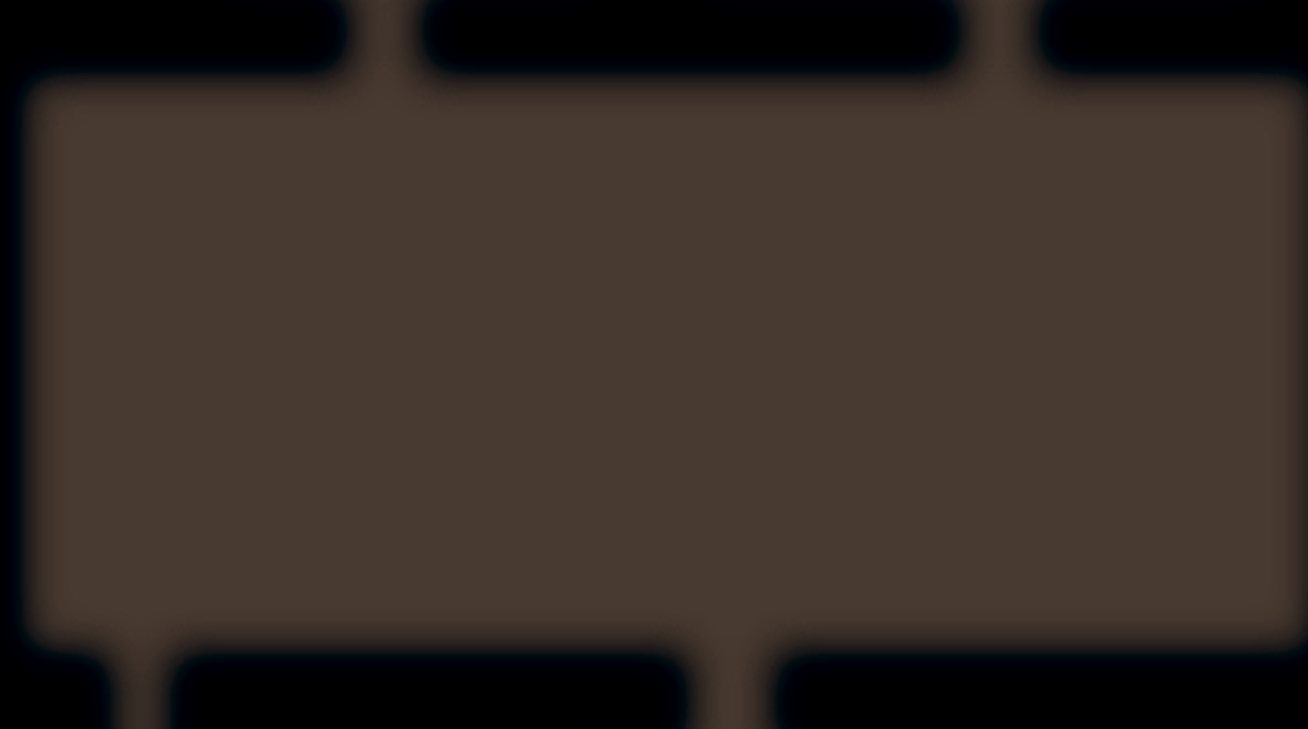
\includegraphics[scale=0.3]{images/nonPaused.png}
	\caption{nonPaused}
	\label{fig:nonPaused}
\end{figure}

\begin{figure}[!ht]
	\centering
	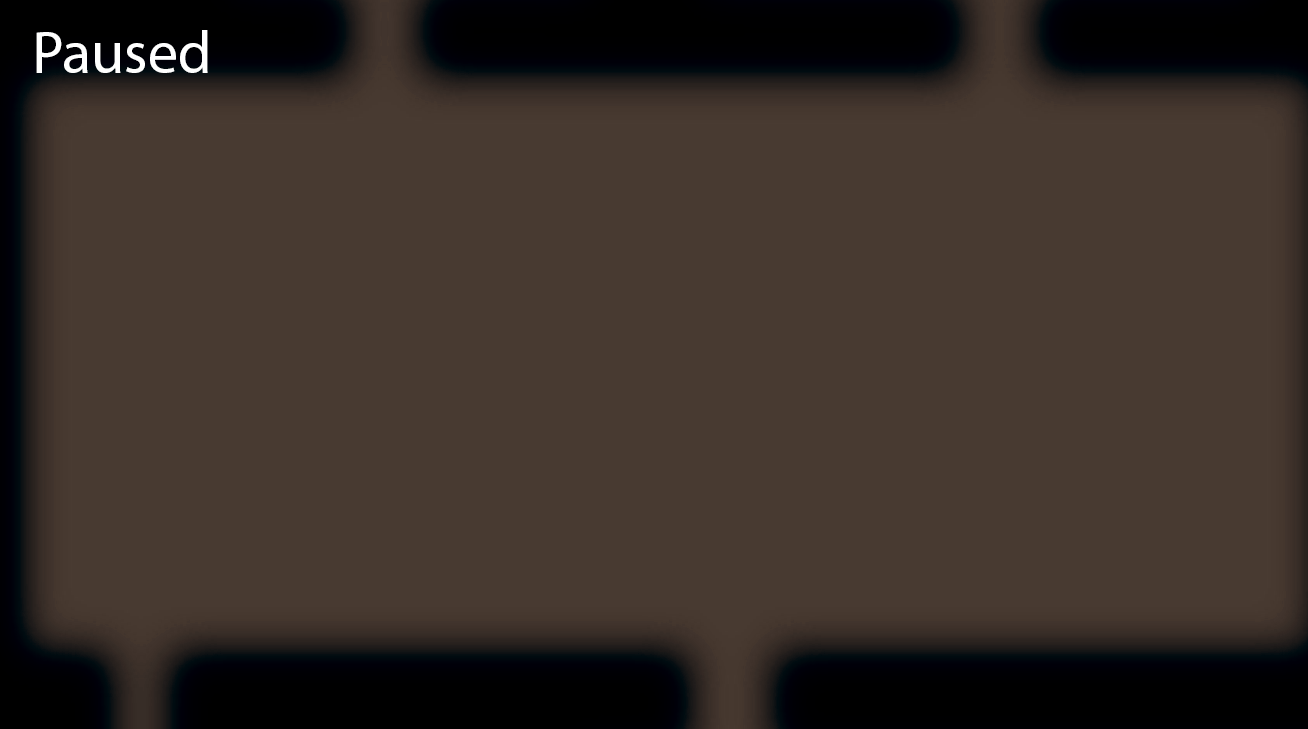
\includegraphics[scale=0.3]{images/Paused.png}
	\caption{Paused}
	\label{fig:Paused}
\end{figure}

\begin{figure}[!ht]
	\centering
	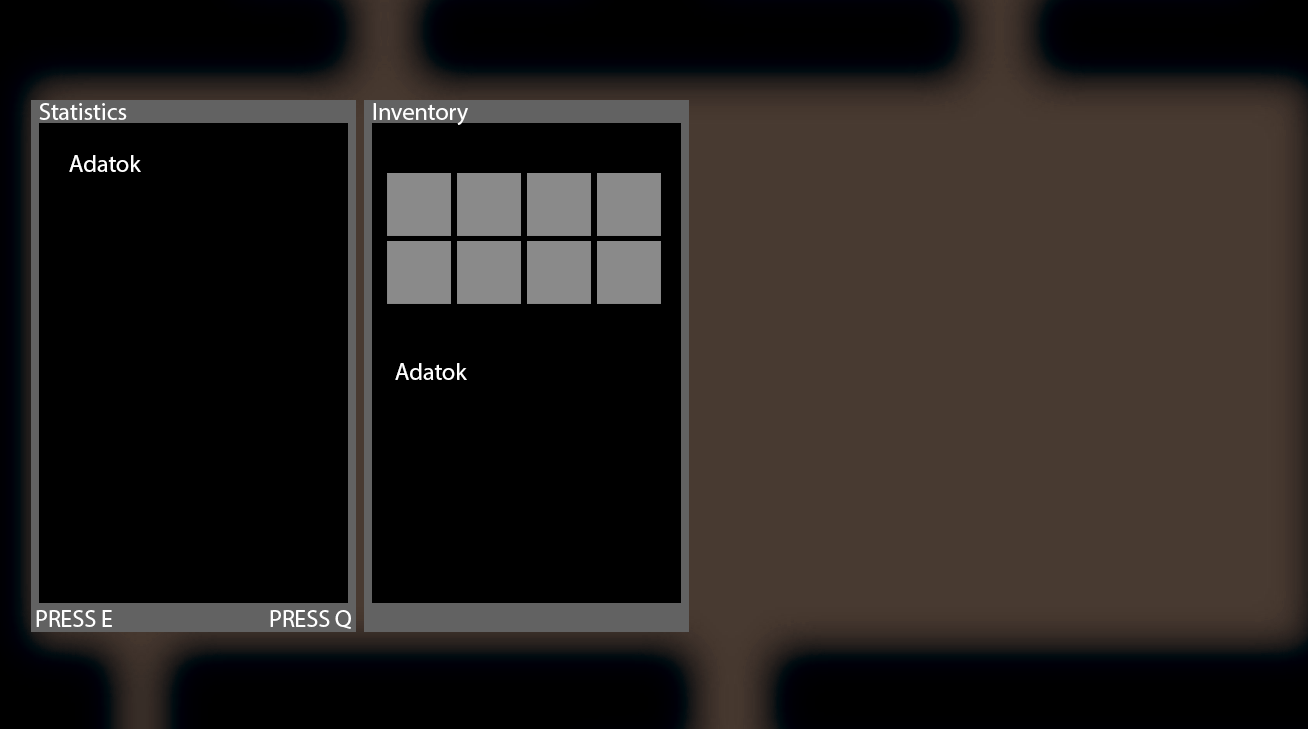
\includegraphics[scale=0.3]{images/Inventory.png}
	\caption{Inventory}
	\label{fig:Inventory}
\end{figure}

\begin{figure}[!ht]
	\centering
	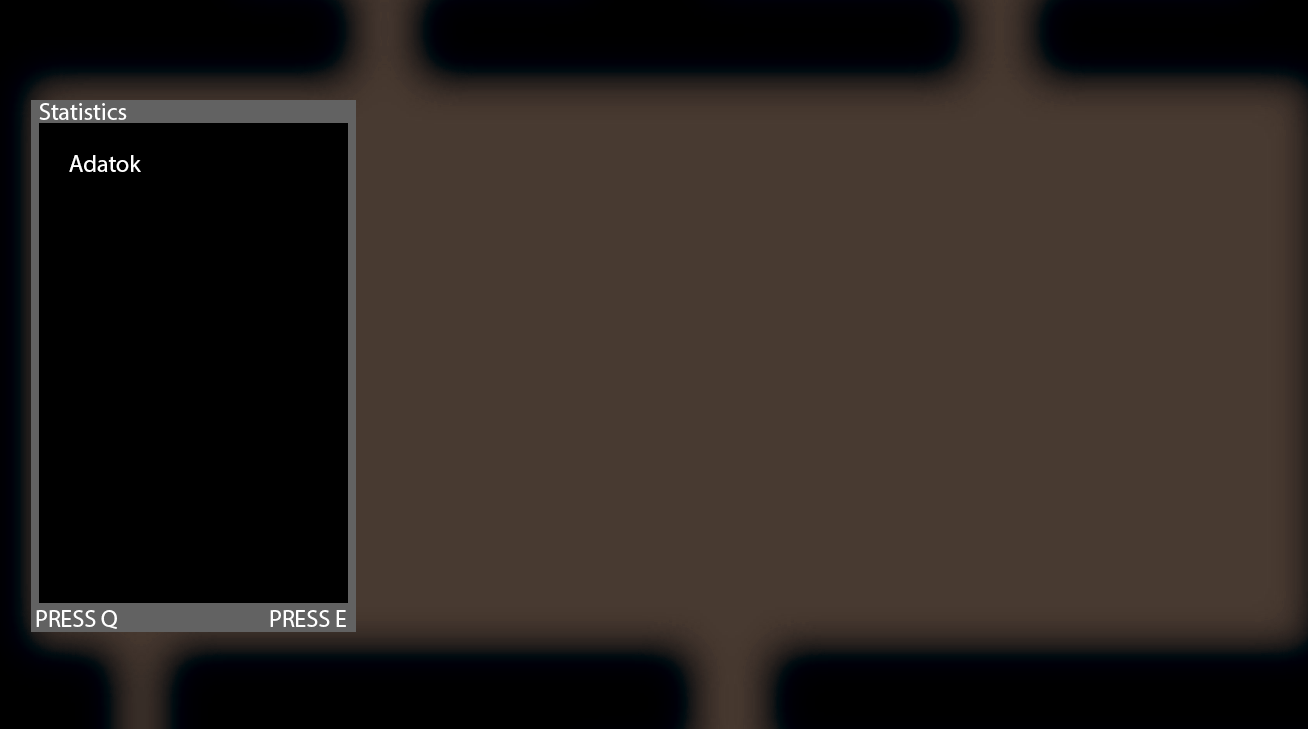
\includegraphics[scale=0.3]{images/Statistics.png}
	\caption{Statistics}
	\label{fig:Statistics}
\end{figure}

\begin{figure}[!ht]
	\centering
	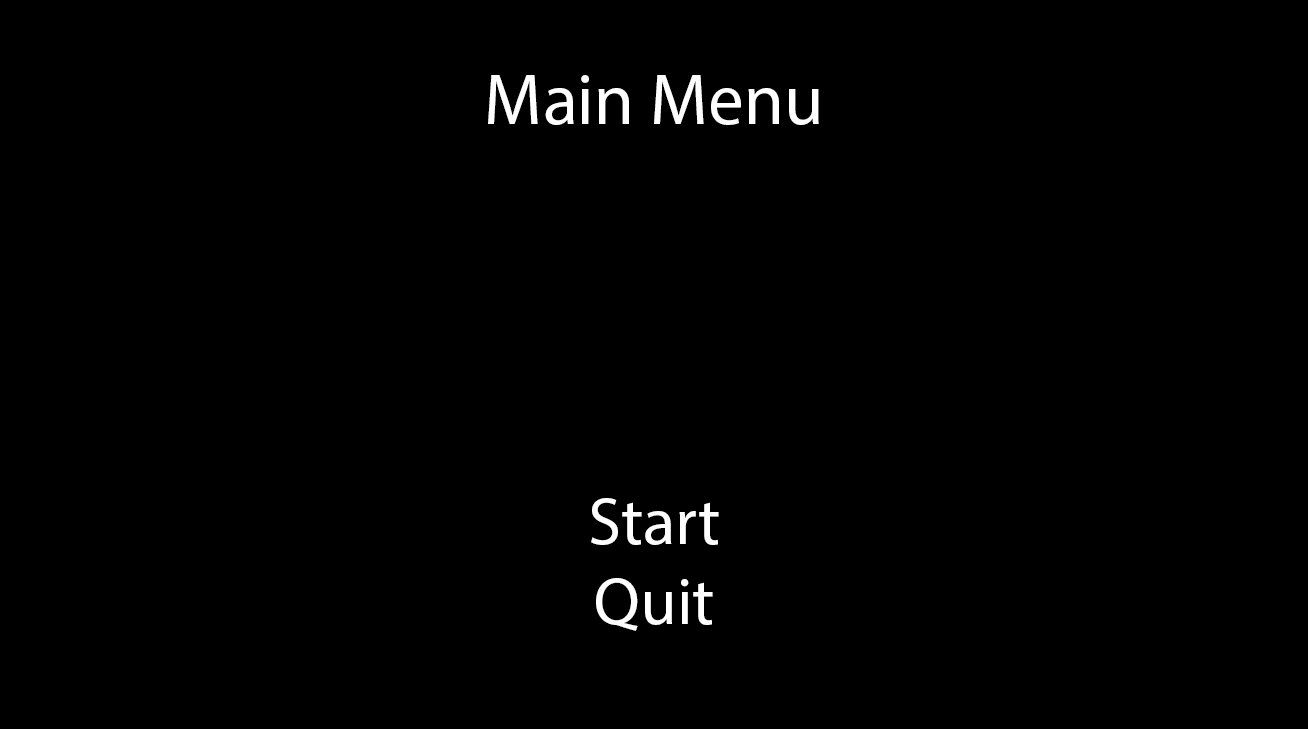
\includegraphics[scale=0.3]{images/MainMenu.png}
	\caption{Main Menu}
	\label{fig:MainMenu}
\end{figure}

\begin{figure}[!ht]
	\centering
	
\includegraphics[scale=0.3]{images/endscreenblue.png}
	\caption{Blue End Screen}
	\label{fig:BlueEndScreen}
\end{figure}

\begin{figure}[!ht]
	\centering
	
\includegraphics[scale=0.3]{images/endscreenred.png}
	\caption{Red End Screen}
	\label{fig:RedEndScreen}
\end{figure}

\begin{figure}[!ht]
	\centering
	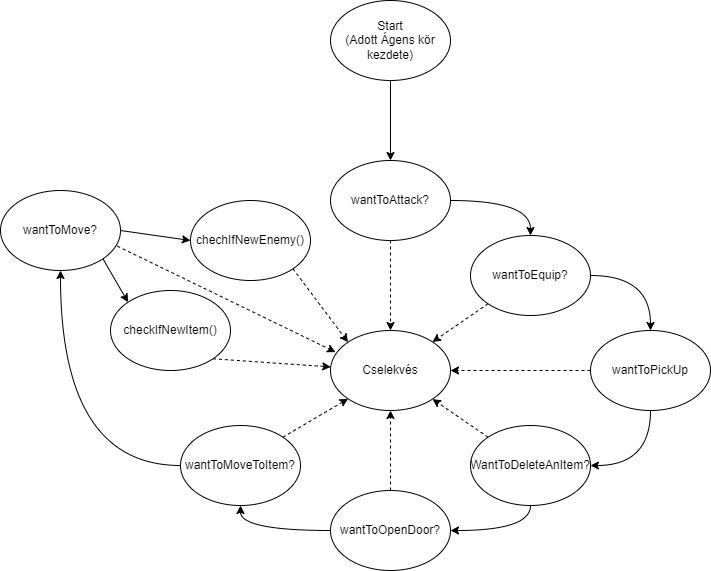
\includegraphics[scale=0.6]{images/agentfunction.png}
	\caption{Agent Action Priority}
	\label{fig:Priority}
\end{figure}

\begin{table}[h!]
    \begin{center}
    \begin{tabular}{ | c | c | c | }
    \hline
    
\includegraphics[width=0.3\textwidth, height=60mm]{images/Entity_Armor_01.png}
    & 
    
\includegraphics[width=0.3\textwidth, height=60mm]{images/Entity_Helmet_01.png}    
    & 
    
\includegraphics[width=0.3\textwidth, height=60mm]{images/Entity_Weapon_01.png}
    \\
    \hline
    
\includegraphics[width=0.3\textwidth, height=60mm]{images/Entity_Armor_02.png}
    & 
    
\includegraphics[width=0.3\textwidth, height=60mm]{images/Entity_Helmet_02.png}    
    & 
    
\includegraphics[width=0.3\textwidth, height=60mm]{images/Entity_Weapon_02.png}
    \\
    \hline
    \end{tabular}
    \caption{Item set 01}
    \label{tbl:Equipable items}
    \end{center}
\end{table}

\begin{table}[h!]
    \begin{center}
    \begin{tabular}{ | c | c | }
    \hline
    
\includegraphics[width=0.3\textwidth, height=60mm]{images/key.png}
    & 
    \includegraphics[width=0.3\textwidth, height=60mm]{images/Door.png}    
    \\
    \hline
    \end{tabular}
    \caption{Key and Door}
    \label{tbl:Key and Door}
    \end{center}
\end{table}

\begin{table}[h!]
    \begin{center}
    \begin{tabular}{ | c | c | c | }
    \hline
    
\includegraphics[width=0.3\textwidth, height=60mm]{images/block_brick.png}
    & 
    
\includegraphics[width=0.3\textwidth, height=60mm]{images/block_grass.png}    
    & 
    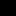
\includegraphics[width=0.3\textwidth, height=60mm]{images/block_empty.png}
    \\
    \hline
    \end{tabular}
    \caption{Blockok}
    \label{tbl:Blocks}
    \end{center}
\end{table}

\begin{table}[h!]
    \begin{center}
    \begin{tabular}{ | c | c | c | }
    \hline
    
\includegraphics[width=0.3\textwidth, height=60mm]{images/chest_0.png}
    & 
    
\includegraphics[width=0.3\textwidth, height=60mm]{images/chest_1.png}    
    & 
    
\includegraphics[width=0.3\textwidth, height=60mm]{images/object_brick.png}
    \\
    \hline
    \end{tabular}
    \caption{Chests and Brick}
    \label{tbl:Chests and Brick}
    \end{center}
\end{table}